 
\documentclass[a4paper,10pt]{article}
\usepackage[utf8x]{inputenc}
\usepackage{graphicx}
\usepackage{fancyhdr}
\usepackage{lastpage}
\usepackage{color}
\definecolor{Blue}{rgb}{0.0,0.0,0.7}
\definecolor{Red}{rgb}{0.7,0.0,0.0}
\definecolor{Green}{rgb}{0.0,0.5,0.0}
\usepackage{hyperref}
\usepackage{ifthen}
\usepackage{algorithm}
\usepackage{algorithmic}
\usepackage{multirow}
\usepackage{textcomp}

%opening
\title{Capacitive Mains Inputs; choosing capacitor and resistor combinations for 120 V a.c. 240 V a.c and 50 and 60Hz}
\author{R.P. clark}

\begin{document}

\maketitle

\begin{abstract}
Calculations to work out capacitance values to drive an opto-coupler to detect mains voltage
for 50 to 60 Hz.
\end{abstract}
\begin{figure}[h]
 \centering
 \includegraphics[width=200pt]{./images_sw_doc/opto.jpg}
 % opto.jpg: 854x388 pixel, 72dpi, 30.13x13.69 cm, bb=0 0 854 388
 \caption{Opto-coupled mains input circuit}
 \label{fig:opto}
\end{figure}

\section{Opto coupler circuit}

This circuit is used to detect mains voltage via a capacitor and a resistor
forming a potential divider so that a lower voltage can be used to drive an opto-isolator
that protects the processor reading the signal.



\section{Calculations}

A potential divider using a capacitor and a resistor is used to lower mains voltage
to levels that can drive a typical opto-coupler input ($\approx 2V$).

A potential divider using a capacitor and resistor means
using the complex identity for the capacitors reactance, $X$.

$$ X = \frac{-j}{\omega C } $$
 
The ${\omega C }$ term is dependent on frequency and is equivalent to $2.\pi.f$ .

Using a potential divider to determine the voltage over the resistor gives:

$$ V_{out} = V_{in} \times \frac{R}{R-\frac{j}{2.\pi.f.C}} $$


The equation above leaves a complex divisor.
To get a complex number as the numerator, the denominator and numerator must be multiplied by
the  conjugate of the denominator, thus:
$$\frac{R}{R-\frac{j}{2.\pi.f.C}} \equiv  \frac{R \times \Big({R+\frac{j}{2.\pi.f.C}}\Big) }{\Big({R-\frac{j}{2.\pi.f.C}}\Big) \times \Big({R+\frac{j}{2.\pi.f.C}}\Big) } $$  

This leaves a real number as the denominator, i.e. $ R^2 + {\frac{1}{2.\pi.f.C}}^2$. 
The resulting complex number, $X$,  
$$X = \frac{R \times \Big({R+\frac{j}{2.\pi.f.C}}\Big) }{R^2 + {\frac{1}{2.\pi.f.C}}^2}$$ 
or,
\begin{equation}
 X =\frac{R^2 + \Big({R\frac{j}{2.\pi.f.C}}\Big) }{R^2 + {\frac{1}{2.\pi.f.C}}^2} 
\label{eqn:genpotdivcapres}
\end{equation}

can now be evaluated for phase and magnitude. Equation~\ref{eqn:genpotdivcapres} can be generally applied to potential dividers
in figure~\ref{fig:opto}.


\subsection{Example calculation}


At 50Hz with 240 V a.c. applied, with R at 1000 Ohms and C at 47 nF

$$\frac{1000^2 + \Big({1000\frac{j}{2.\pi.50.47e-9}}\Big) }{R^2 + {\frac{1}{2.\pi.50.47e-9}}^2}$$
$$\frac{1000^2 + \Big({1000 \times 67726j}\Big) }{1000^2 + {67726}^2}$$
$$\frac{1000^2 + \Big({67726000j}\Big) }{4.5877 \times 10^9}$$

This gives a complex number $$ \frac{1000^2 + {67726000j} }{4.5877 \times 10^9}$$ i.e. $$(216 \times 10^{-6} + 14.76\times 10^{-3} j ) \;.$$
This complex number has a magnitude of 0.0147 and an argument of 89.15 degrees (which is expected as most of the reactance comes from the capacitor).
So with 240 V a.c. applied (RMS) the opto would see a signal with $0.0147*240 = 3.54V (RMS)$
\clearpage
\section{ploting the voltage at the opto-coupler}

\begin{figure}[h]
 \centering
 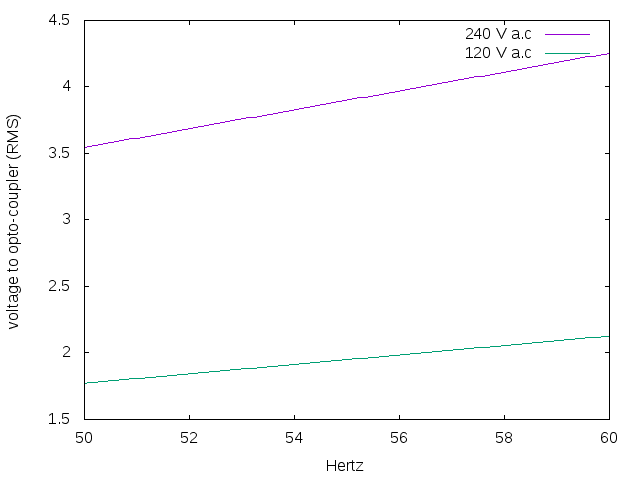
\includegraphics[width=400pt]{./RMS_volts_to_opto.png}
 % RMS_volts_to_opto.png: 640x480 pixel, 72dpi, 22.58x16.93 cm, bb=0 0 640 480
 \caption{RMS voltage seen at opto-coupler for 50 to 60 Hz range}
 \label{fig:rmstoopto}
\end{figure}


\clearpage

\subsection{plotting the voltage at the opto-coupler: gnuplot scripts}
 
{ \tiny
\begin{verbatim}
########################################################
#
p=3.14159265358979323844
#
# 47nF
C=47e-9
#
# 1k Ohms
R=1000

# define complex operator
j={0,1}

set xlabel "Hertz"
set ylabel "Resistance"

# x is the frequency
set xrange[50:60]

# z(x) is the reactance
z(x)=(j/(2*p*x*C))

# denominator
d(x)=(R*R+z(x)*z(x))

# numerator
n(x)=(R*R+R*z(x))

plot abs(z(x)) title "reactance over capacitor"
!sleep 4

set ylabel "denominator value (abs)"
plot abs(d(x))
!sleep 4

set ylabel "numerator value (abs)"
plot abs(n(x))
!sleep 4

v(x)=abs((n(x))/(d(x)))

# gives large numbers h(x)=arg((n(x))/(d(x)))

set ylabel "voltage to opto-coupler (RMS)"
plot 240*v(x) title "240 V a.c", 120*v(x) title "120 V a.c"
!sleep 4

set terminal png
set output "RMS_volts_to_opto.png"
plot 240*v(x) title "240 V a.c", 120*v(x) title "120 V a.c"

#set angles degrees
#set label "phase change in mains over opto"
#plot 240*h(x) title "240 V a.c", 120*h(x) title "120 V a.c"
#!sleep 4
#
\end{verbatim}


}
% 
% 
% Putting some numbers in this, 47nF for the capacitor, 1k for R and 50 Hz at 240V, means ${2.\pi.f.C} = 14.765 \times 10^{-6}$.
% 
% $$ V_{out} = 240 \times \frac{1000}{ 1000 - \frac{j}{14.765 \times 10^{-6}} } $$
% or
% % $$ V_{out} = 240 \times \frac{1000}{1000 - j  \times  67.726 \times 10^3 }$$
% % % 
% % To get a complex number as the numerator, the denominator and numerator must be multiplied by
% % its conjugate, thus:
% % % 
% % $$\frac{1000}{1000 - {j}  \times  67.726 \times 10^3 } $$
% % % $$
% % % 
% %  \equiv   \frac{ 1000 \times  (1000 + {j}  \times  67.726 \times 10^3) }{ (1000 - {j}  \times  67.726 \times 10^3) \times (1000 + {j}  \times  67.726 \times 10^3)}   $$
% % $$
% 
typeset in {\Huge \LaTeX} \today.
 \end{document}
